% !TEX encoding = UTF-8 Unicode

\Chapter{Szűrő algoritmusok}

Ebben a fejezetben azokat a filtereket részletezem, amelyeket C++ programozási nyelven készítettem el. Többségükben rajzfilm, valamint festmény jellegűek. A szűrőket nem csak képeken teszteltem, hanem videókon is és valós időben is a számítógépem kamerájával. (Az utóbbiak eredményeit \aref{chap:tests}. fejezet részletezi.)

\Section{Cartoon-style filter}

Az első filter egy rajzfilm jellegű (\textit{cartoon-style}) filter, amely az éleket kiemeli és a színeket elmossa. A szűrőhöz az ötletet Michael Beyeler hasonló szűrője adta, melyet Python nyelven készített el \cite{beyeler}.

A műveletekhez Gauss-piramist, kétoldalú szűrést, medián szűrést, illetve adaptív küszöbölést használtam. A szűrés eredményére egy példát \aref{fig:cartoon1}. ábrán láthatunk.

\begin{figure}[ht]
\centering
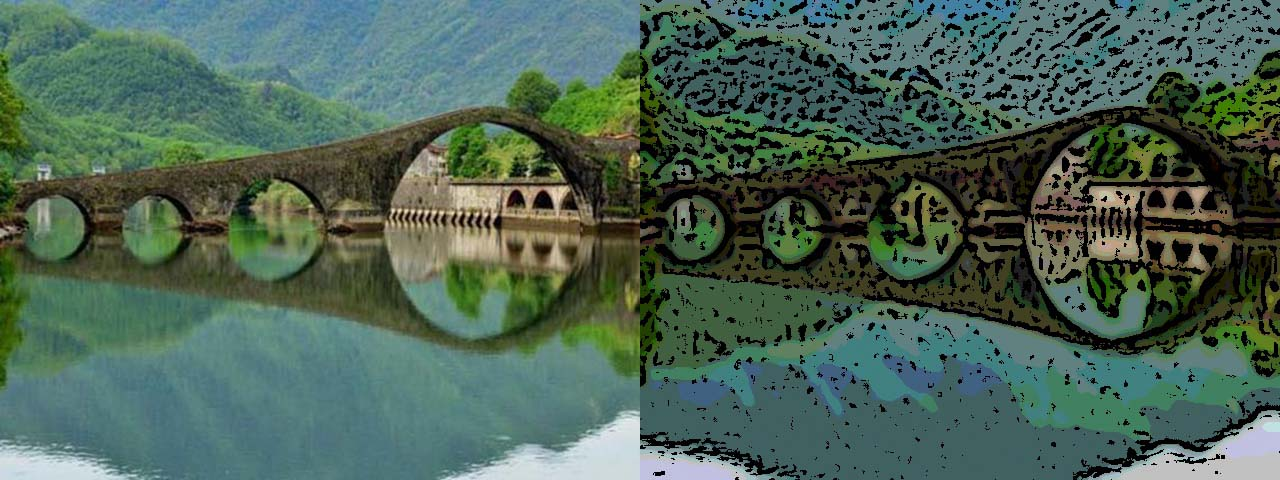
\epsfig{file=kepek/1_cartoon_filter.jpg, width=15cm, height=5.625cm}
\caption{Bal oldalon az eredeti-, jobb oldalon pedig a filterrel ellátott kép látható} 
\label{fig:cartoon1}
\end{figure}

\SubSection{Gauss-piramis és kétoldalú szűrő}

Első lépésben az eredeti képet lekicsinyítettem Gauss-piramis segítségével a kép méretének negyedére, rátettem egy kétoldalú szűrőt, majd vissza nagyítottam az eredeti méretre. A Gauss-piramis a kép kicsinyítése előtt Gauss-simítás segítségével súlyoz. A kétoldalú szűrő egy nem lineáris, élvédő és zajcsökkentő simító szűrő. Ezen lépés eredménye látható \aref{fig:cartoon2}. ábrán.

\begin{figure}[ht]
\centering
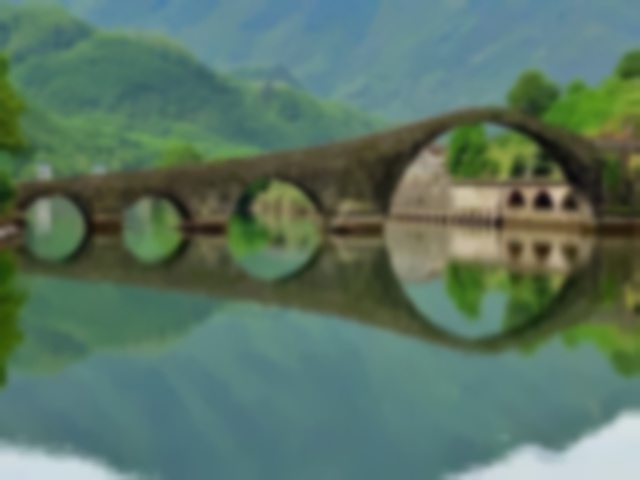
\epsfig{file=kepek/pyrambilateral.jpg,scale=0.45}
\caption{A Gauss-piramisban kicsinyítés és nagyítás valamint a kétoldalú szűrő eredménye } 
\label{fig:cartoon2}
\end{figure}

\SubSection{Színek konvertálása, medián szűrő}

Ebben a lépésben először az előzőleg kapott elmosott, színes képet átkonvertáltam szürkeárnyalatos képpé. 
Itt ki szeretnék térni magára a színes kép szürkeárnyalatossá konvertálására. Több féle megoldás létezik, ebből az elterjedtebbeket említeném. Az egyik az RGB komponensek átlagolása, de ez az emberi szem számára pontatlan, mivel nem egyformán érzékelünk minden színt. A következő lehetőség, amit az OpenCV- beépített színkonvertálása is használ az, hogy a komponensek súlyozott átlagát veszi, de nem egyenlő súlyértékekkel. Ennek a speciális esete, amely a HSV színrendszer \textit{value} értékét számítja. Ebben az esetben az OpenCV-s beépített kovertálást használtam a következő súlyokkal:
$$
\text{RGB to Gray} = 0.299 \cdot R+0.587 \cdot G + 0.114 \cdot B.
$$ 
Ennek eredményeként kapott képen medián szűrést hajtottam végre, amit ismét zajcsökkentés miatt alkalmaztam. Így a kép már teljesen el van mosva, egyre jobban rajzfilmszerű hatása van. Ennek az eredménye \aref{fig:cartoon3}. ábrán látható.

\begin{figure}[ht]
\centering
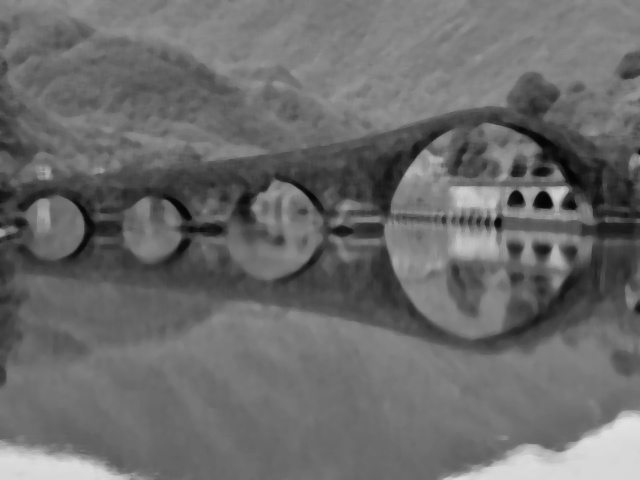
\epsfig{file=kepek/graymedian.jpg,scale=0.45}
\caption{Szürkére átalakított kép medián szűrővel} 
\label{fig:cartoon3}
\end{figure}

\newpage

\SubSection{Adaptív küszöbölés az élek kiemelésére}

Az adaptív küszöbérték általában szürkeárnyalatos vagy színes képet kap bemenetként, és a legegyszerűbb megvalósításban bináris képet eredményez. A kép minden egyes képpontjára egy küszöbértéket kell kiszámítani. Ez a küszöbérték lehet például egy kernelen belüli intenzitások átlaga, vagy egy, a hisztogram alapján becsült érték. Amennyiben a képpontérték a küszöbérték alatt van, akkor a háttérértékre van állítva, ellenkező esetben az előtérbe kerül.

\begin{figure}[ht]
\centering
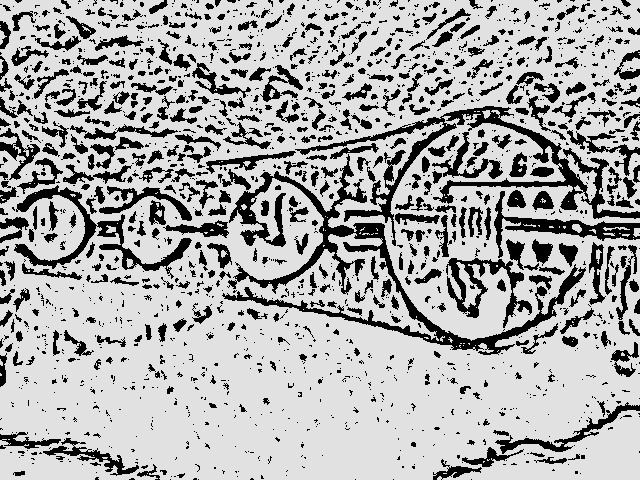
\epsfig{file=kepek/threshold.jpg,scale=0.40}
\caption{Az adaptív küszöbölés eredménye} 
\label{fig:cartoon4}
\end{figure}

\SubSection{A szűrőkkel és a küszöböléssel előállított képek egyesítése}

Az adaptív küszöböléssel elkészült maszkot át kell konvertálni színes képpé, hogy egyesíteni tudjuk az "elmosott" képpel amit az első két lépésben hoztunk létre. Ennek az elvégzését követően \aref{fig:cartoon5}. ábrán látható eredményt kaptuk.

\begin{figure}[ht]
\centering
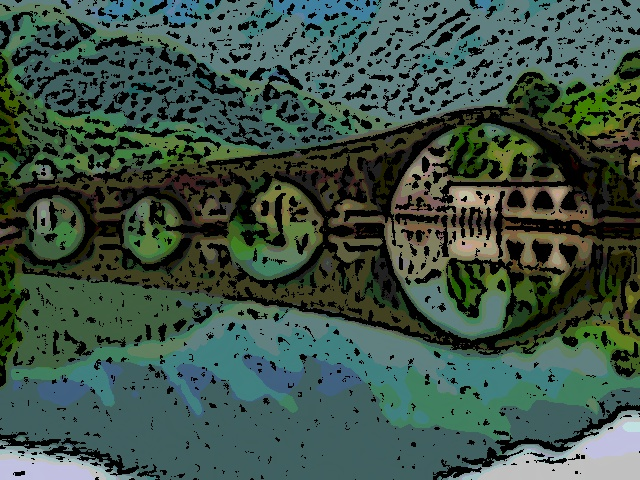
\epsfig{file=kepek/Cartoon_filter.jpg,scale=0.40}
\caption{Cartoon-style szűrő } 
\label{fig:cartoon5}
\end{figure}

% TODO: Esetleg pontszerű zajok eltávolítási módjáról lehet még néhány dolog a binarizált kép esetében.

\Section{Pencil sketch filter}

% https://github.com/MasteringOpenCV/code/blob/master/Chapter1_AndroidCartoonifier/Cartoonifier_Desktop/cartoon.cpp

Megpróbáltam egy olyan algoritmust létrehozni, ami egy ceruza rajzot imitál. A szakirodalomban találunk hasonló szűrési eljárásokat, mivel egy gyakran előforduló hatásról van szó \cite{emami}.

A feldolgozáshoz szűrkeárnyalatosra konvertáltam a képet, medián szűrőt, Gauss szűrőt és egyéb képfeldolgozási műveleteket használtam, valamint egy "vásznat" is ráraktam, hogy még jobban olyan érzete legyen a képnek mint ha rajzolták volna (\ref{fig:pencil1}. ábra).

\begin{figure}[ht]
\centering
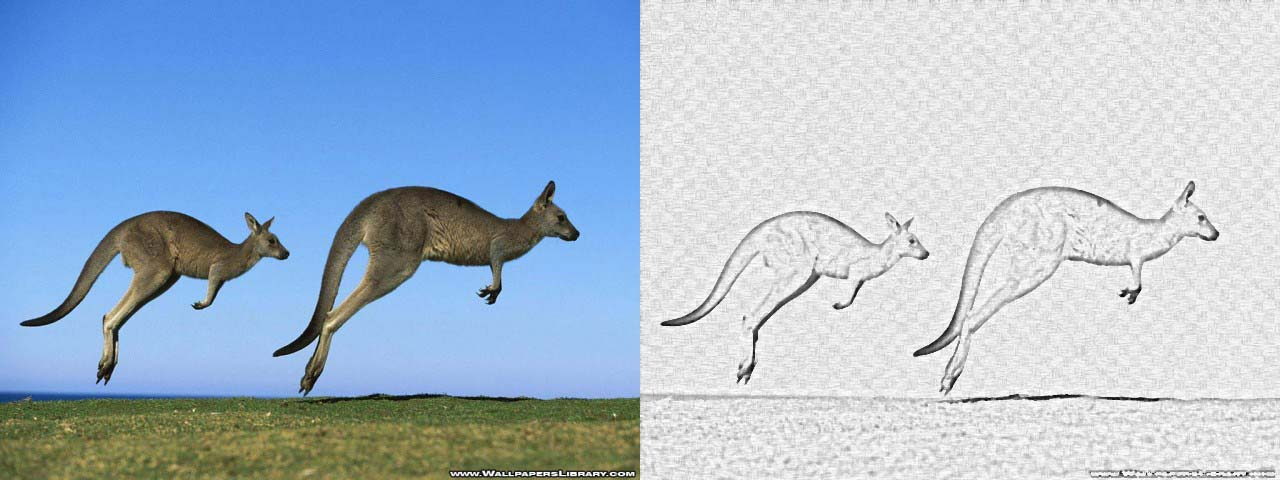
\epsfig{file=kepek/2_pencil_sketch_filter.jpg,width=15cm, height=5.625cm}
\caption{Bal oldalon az eredeti kép látható, jobb oldalon a filterrel ellátott kép} 
\label{fig:pencil1}
\end{figure}

\SubSection{Medián szűrő}

A kép szűrkeárnyalatos konvertálása után, végrehajtottam egy medián szűrést a kisebb, pont szerű zajok eltávolítása céljából (\ref{fig:pencil2}. ábra). A kernel méretétől függően már ez ad egy egyhe elmosást is a képhez, amely a végeredmény szempontjából előnyös.

\begin{figure}[ht]
\centering
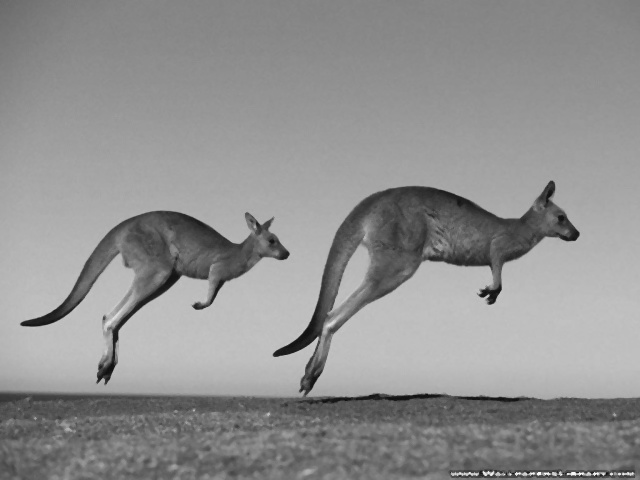
\epsfig{file=kepek/mediangray.jpg,scale=0.50}
\caption{Szürkére átalakított kép medián szűrővel} 
\label{fig:pencil2}
\end{figure}

\SubSection{Gauss szűrő}

Ezt a simítási teknikát, a képzaj  és a részletesség csökkentése érdekében használtam. Olyan sima elmosódást eredményez a képen, mint ha az nem lenne fókuszban (\ref{fig:pencil3}. ábra). A medián szűrőhöz képest lényeges különbség, hogy ezzel új árnyalatok is megjelennek a képen, a kontraszt összességében csökken.

\begin{figure}[ht]
\centering
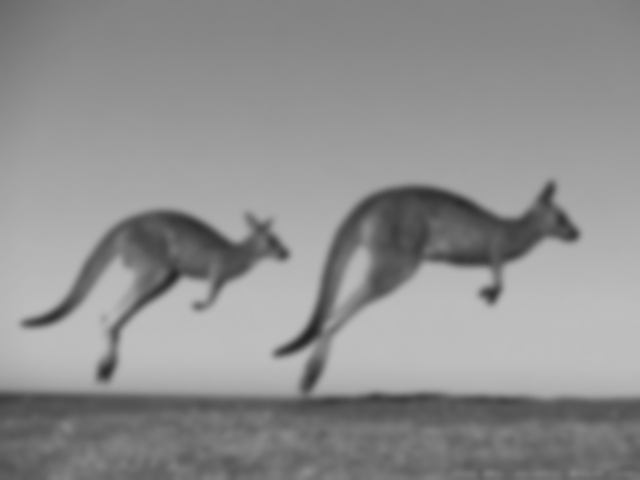
\epsfig{file=kepek/gauss.jpg,scale=0.43}
\caption{Gauss szűrő használata } 
\label{fig:pencil3}
\end{figure}

\SubSection{Az előző két lépés elosztása}

% TODO: Az osztást itt részletezni kicsit!

Az előző két szűrőt elosztottam egymással, így már tényleg majdnem olyan képet kaptam ami már ceruza rajz szerű. Úgy gondoltam még azért ráfér némi javítás, így még további műveleteket hajtottam végre rajta.

\begin{figure}[ht] 
\centering
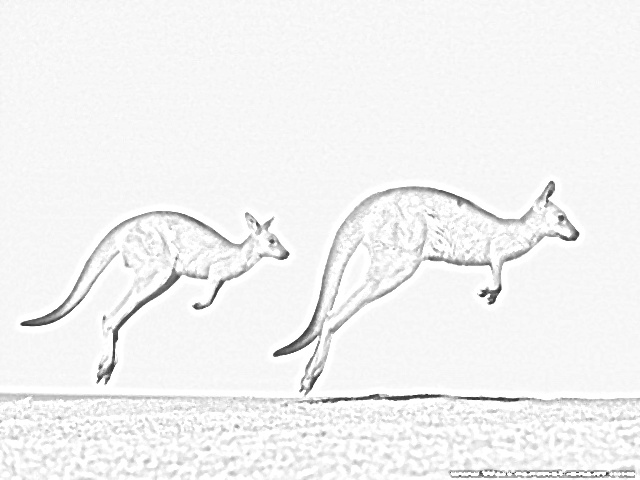
\epsfig{file=kepek/blend.jpg,scale=0.43}
\caption{Medián szűrés és a Gauss szűrés hányadosa } 
\label{fig: pencil4}
\end{figure}

\SubSection{Kontraszt széthúzása}

Azt figyeltem meg, hogy ha így hagyom a "Pencil sketch" szűrőt, akkor némely kép eléggé kontraszt szegény marad. Emiatt célszerűnek tünt belerakni egy kontraszt széthúzást, a szebb végeredmény érdekében. A széthúzás (vagy másnéven \textit{normalizáció}) egy egyszerű képjavító eljárás, amely megpróbálja javítani a kép kontrasztját azáltal, hogy "kiterjeszti" a benne lévő intenzitásértékek tartományát a kívánt értéktartományra. Ezt a műveletet követően a példaként szereplő képre \aref{fig:pencil5}. ábrán látható eredményt kaptam.

\begin{figure}[ht]
\centering
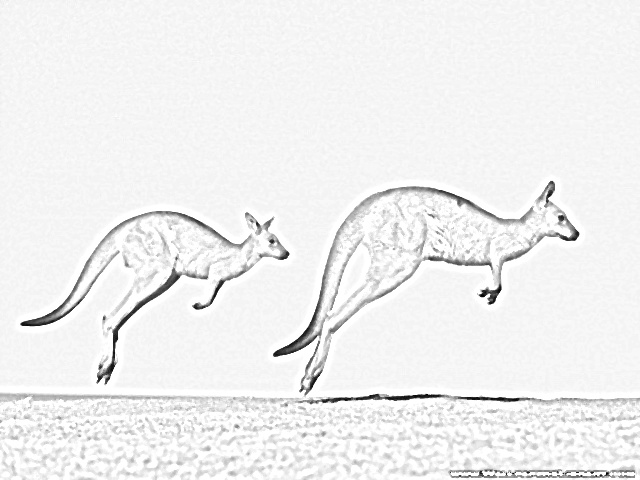
\epsfig{file=kepek/contraststrech.jpg,scale=0.50}
\caption{Kontraszt széthúzás} 
\label{fig:pencil5}
\end{figure}

\SubSection{Vászon hozzáadása}

A kontraszt széthúzása után, már egészen olyan hatása volt a képnek, mint ha egy ceruza rajz lenne. Ráraktam még egy "vászont" ami személyes véleményem szerint mégjobban segíti azt az érzetet hogy ez egy ceruzarajz. Először a vászonnak a színét át kellett konvertálnom színesből szűrkeárnyalatossá, hogy használható legyen a kontraszt széthúzott képhez (\ref{fig:pencil6}. ábra). Ezek után a vászont összeszoroztam az eddig eredményül kapott képpel, így jött létre a "Pencil sketch filter".

\begin{figure}[ht] 
\centering
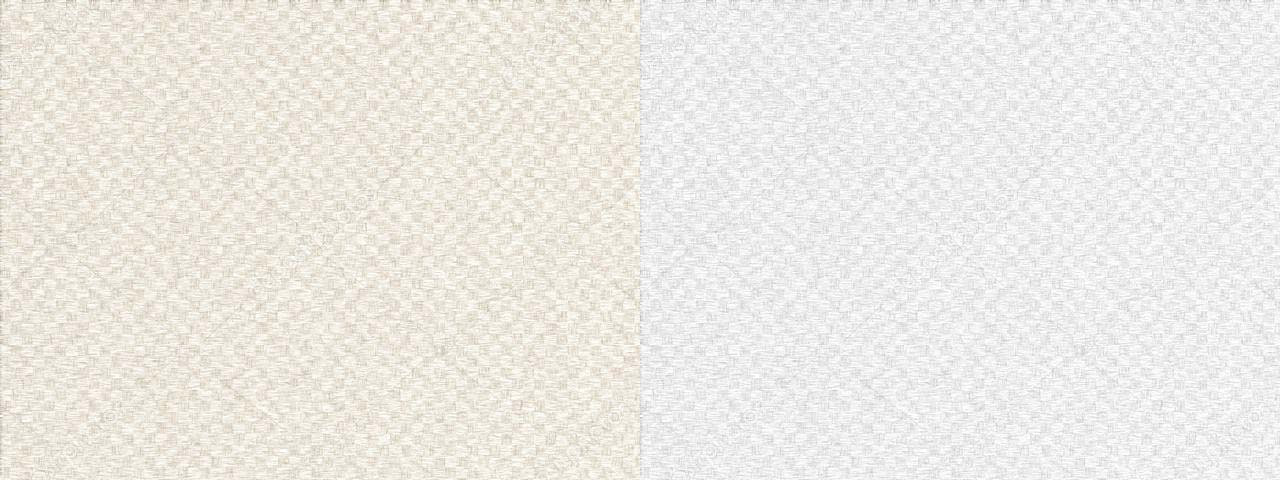
\epsfig{file=kepek/canvasgray.jpg,width=10cm, height=3cm}
\caption{Vászon színének konvertálása}
\label{fig:pencil6}
\end{figure}

\Aref{fig:pencil7}. ábrán láthatjuk a végeredményként kapott képet.

\begin{figure}[ht]
\centering
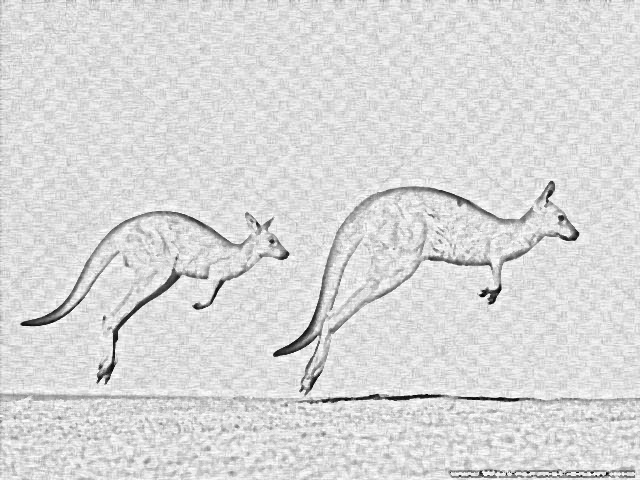
\epsfig{file=kepek/pencil_sketch.jpg, scale=0.50}
\caption{A \textit{Pencil sketch filter} eredménye} 
\label{fig:pencil7}
\end{figure}

\Section{Cartoon filter}

Megpróbáltam más technikával is létrehozni egy cartoon hatású képet. Ahol medián szűrőt, Laplace éldetektálást valamit küszöbölést használtam (\ref{fig:2_cartoon1}. ábra).

\begin{figure}[ht]
\centering
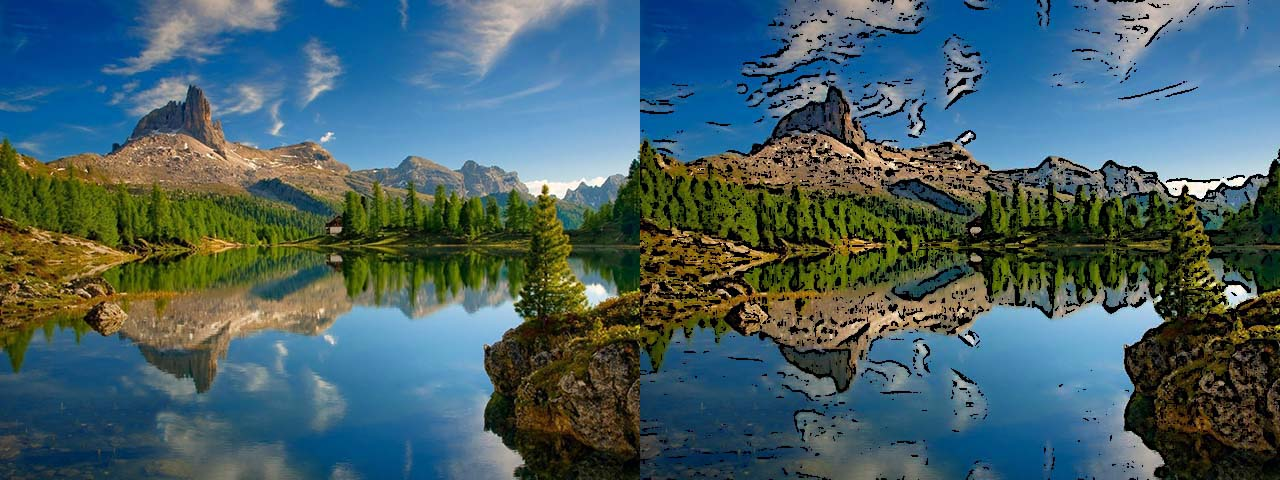
\epsfig{file=kepek/3_cartoon_filter2.jpg,width=15cm, height=5.625cm}
\caption{Bal oldalon az eredeti kép látható, jobb oldalon a filterrel ellátott kép} 
\label{fig:2_cartoon1}
\end{figure}

\SubSection{Medián szűrő}

Mint az eddigi saját filtereknél, itt is előfeldolgozásként elvégeztem szürkeárnyalatossá konvertálást valamint egy medián szűrést (\ref{fig:2_cartoon2}. ábra).

\begin{figure}[ht]
\centering
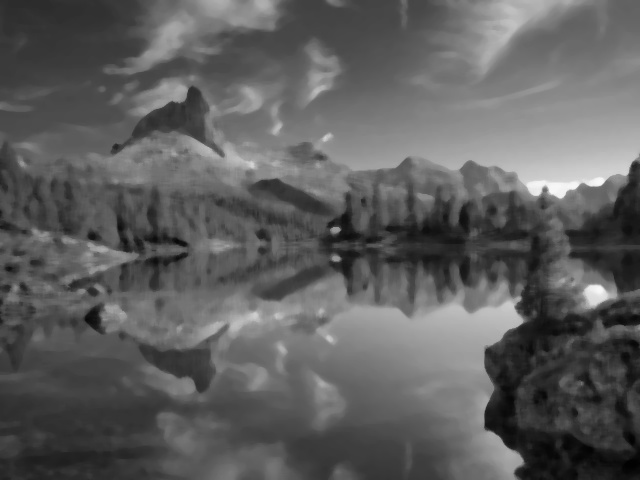
\epsfig{file=kepek/Cartoon1_gray.jpg,scale=0.485}
\caption{Szürkére átalakított kép medián szűrővel} 
\label{fig:2_cartoon2}
\end{figure}

\SubSection{Laplace éldetektálás}

Ennél a filternél a Laplace éldetektálást választottam. Ezzel olyan élmaszkot tudtam készíteni, amely kicsit hasonló a ceruza rajzhoz. Vékony kontúrként emeli ki a képben található éleket (\ref{fig:2_cartoon3}. ábra).

% Ez az éldetektálás gradiensekkel számol, ahol a gradiens nagy, ott a második derivált értéke 0.

\begin{figure}[ht]
\centering
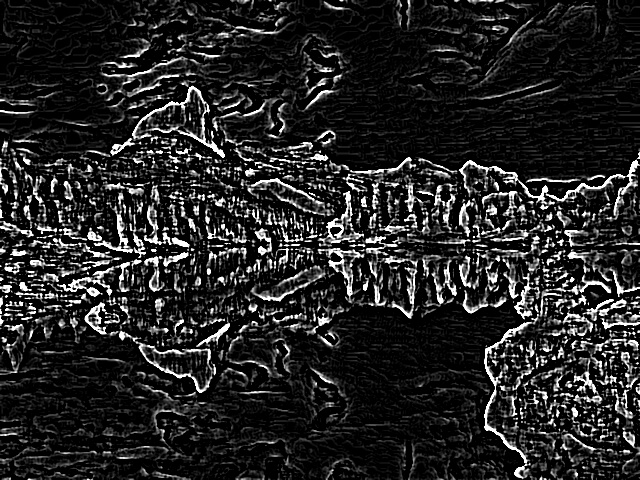
\epsfig{file=kepek/Cartoon1_laplacian.jpg,scale=0.485}
\caption{Laplacian éldetektálás} 
\label{fig:2_cartoon3}
\end{figure}

\SubSection{Küszöbölés}

Az éldetektálás után, alkalmaztam egy küszöbölést amivel létrejött egy maszk, amit összeraktam az eredeti képpel (\ref{fig:2_cartoon4}. ábra).

\begin{figure}[ht]
\centering
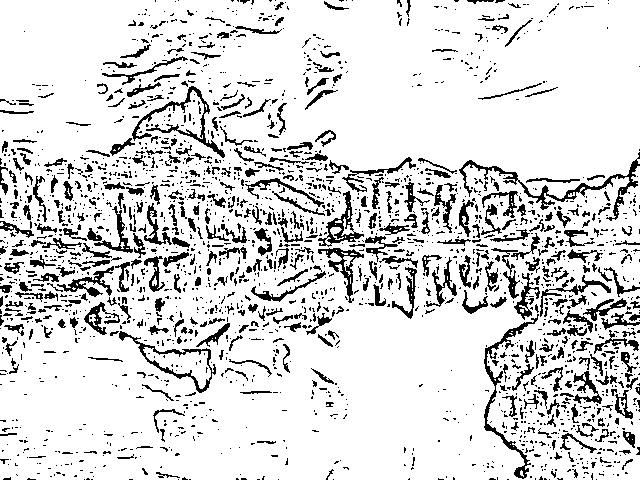
\epsfig{file=kepek/Cartoon1_thresh.jpg,scale=0.4}
\caption{Küszöbölés} 
\label{fig:2_cartoon4}
\end{figure}

Így készült el végeredményként a \textit{Cartoon filter}, melynek az eredménye \aref{fig:2_cartoon5}. ábrán látható.

\begin{figure}[ht]
\centering
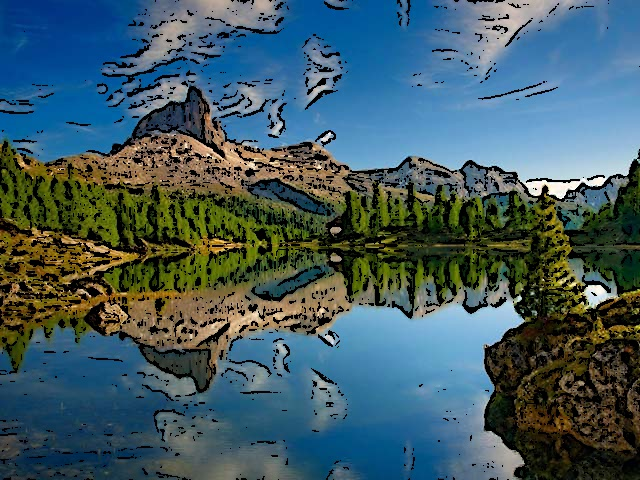
\epsfig{file=kepek/Cartoon1_filter1.jpg,scale=0.48}
\caption{Cartoon filter} 
\label{fig:2_cartoon5}
\end{figure}

\Section{Aquarelle-style filter}

Az utolsó saját szűrő amit készítettem az egy egyszerű vízfesték (\textit{aquarell}) hatású szűrő. Ez a szűrő teljesen más technikával készült mint az eddigiek. Nem használtam éldetektálást illetve küszöbölést sem. Az eredeti képpel dolgoztam végig, nem maszkoltam. A szűrés két lépésben megoldhatónak bizonyult. Elég egy átlagoló szűrés és egy mean shift szegmentálás egymást követően alkalmazni (\ref{fig:paint}. ábra).

\begin{figure}[ht]
\centering
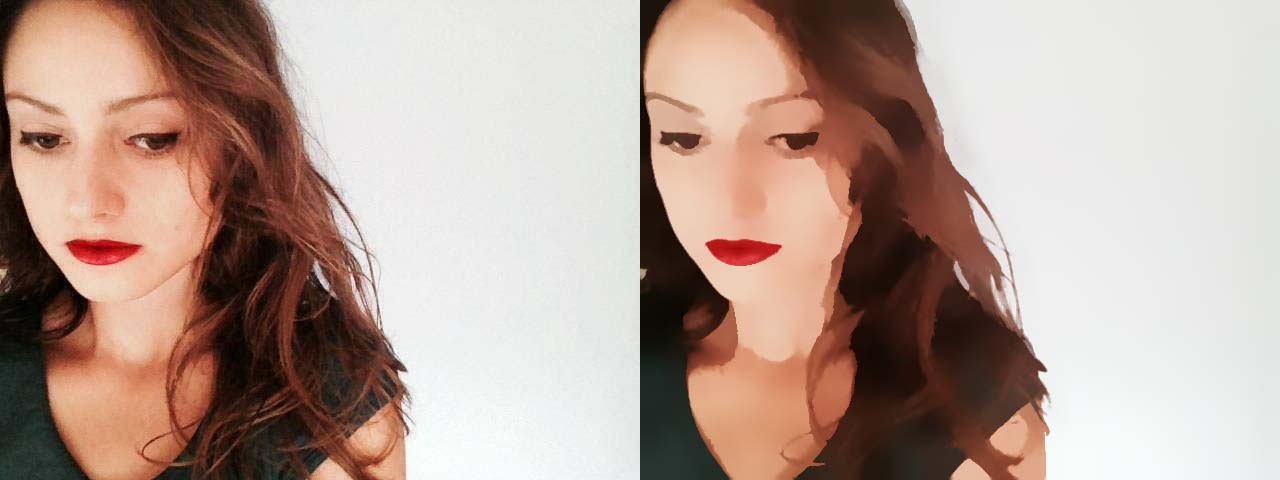
\epsfig{file=kepek/4_paint_filter.jpg,width=15cm, height=5.625cm}
\caption{Aquarelle-style filter} 
\label{fig:paint}
\end{figure}

\SubSection{Átlagoló szűrő}

Átlagoló szűrővel elmostam az eredeti színes képet, hogy az apróbb zajokat kiszűrjem (\ref{fig:paint1}. ábra).

\begin{figure}[ht]
\centering
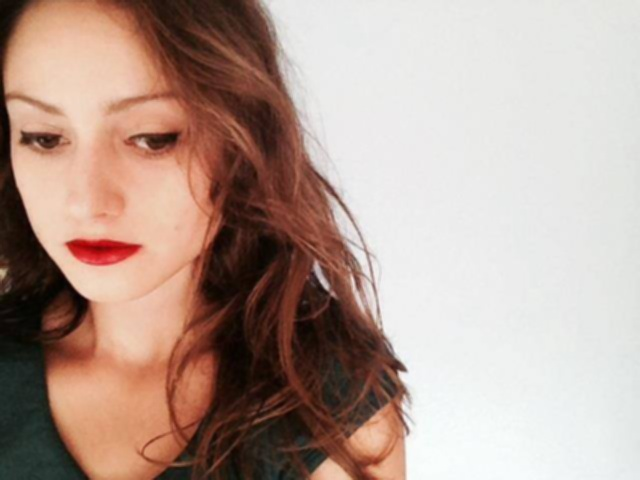
\epsfig{file=kepek/Paint_filter_blur.jpg,scale=0.48}
\caption{Átlagoló szűrő  } 
\label{fig:paint1}
\end{figure}

\SubSection{Mean shift szegmentálás}

Minden egyes adatpontnál a mean shift meghatároz egy ablakot, és kiszámítja az adatpont átlagát. Ezután az ablak közepét az átlag felé tolja, és megismétli az algoritmust, amíg konvergens. Az mean shift egy nemparametrikus iteratív algoritmus vagy egy nemparametrikus sűrűségi gradiens becslés egy általánosított kernel megközelítés alkalmazásával (\ref{fig:paint2}. ábra).

\begin{figure}[ht]
\centering
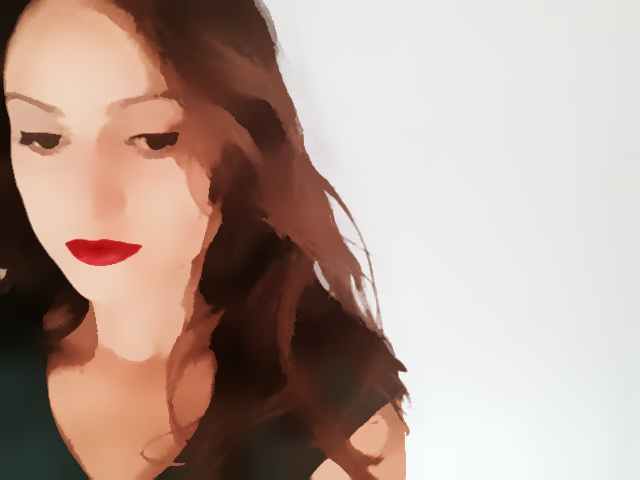
\epsfig{file=kepek/Paint_filter.jpg,scale=0.48}
\caption{Aquarelle-style filter, mean shift szegmentálás  eredménye} 
\label{fig:paint2}
\end{figure}

% https://gist.github.com/dgym/5532135
% Ide kellene felsorolni majd a saját szűrők algoritmusait!
